\chapter{ Fundamentação Teórica} \label{cap2}
Neste capítulo serão apresentados conceitos necessários para o entendimento do trabalho.

\section{Identificação de Sistemas e Estimação de Parâmetros}
A identificação do sistema é o primeiro passo para o seu controle. Nesta seção serão tratados conceitos de identificação de sistemas e estimação de parâmetros fundamentais para o entendimento do trabalho.

\subsection{Visão Geral}
A identificação de sistemas e estimação de parâmetros se tratam de métodos e práticas que permitem construir modelos dinâmicos de um sistema real à partir de experimentos. Muitas vezes um sistema construído que precisa ser controlado não pode ser modelado devido à limitações matemáticas ou imprecisão na interação dos componentes. Nestes casos se utiliza da identificação de sistemas para obter um modelo matemático. A identificação de sistemas se baseia em testar a resposta do sistema à certas entradas e a partir das respostas aproximar o modelo matemático de forma satisfatória. Para identificar sistemas temos métodos determinísticos, que desprezam o ruído presente nos dados, e métodos não paramétricos, que não resultam em um modelo matemático mas em uma representação gráfica da dinâmica do sistema da qual um modelo pode ser extraído.


\subsection{Identificação por Mínimos Quadrados}
O método de mínimos quadrados é um dos mais conhecidos e utilizados em várias áreas da ciência e tecnologia. Ele utiliza sistemas de equações com matrizes geradas a partir de testes com os sistemas reais no seguinte formato:
\begin{equation}
	\hat{\Theta}=[X^TX]^{-1}X^Ty
\end{equation}
A equação 2.1 é o objetivo da identificação por quadrados mínimos, mas para entender ela precisamos primeiro entender de onde ela vem.
\newline 
Um sistema geralmente é descrito por uma função entrada - saída, em um sistema onde não sabemos a função podemos executar uma série de testes para obtermos um conjunto de valores de entrada e saída da seguinte forma:
\begin{equation}
\begin{array}{c}
y_1=f(x_1) \\
y_2=f(x_2) \\
y_3=f(x_3) \\
... \\
y_N=f(x_N)
\end{array}
\end{equation}
Podemos então tratar esse conjunto como vetores da seguinte forma:
\begin{equation}
y=f(x,\Theta)
\end{equation}
Existem três considerações que devem ser tomadas para avançar o entendimento de mínimos quadrados.
\begin{enumerate}
	\item A função f e o vetor $\theta$ não variam de uma restrição para outra. Todas as restrições são da mesma equação. Em problemas de identificação de sistemas dinâmicos normalmente supõe-se que o sistema seja invariante no tempo e que os sinais medidos sejam estacionários, caso não fossem f e $\theta$ seriam diferentes entre restrições complicando a estimação de um único f e um único $\theta$.
	\item A equação 2.3 pode ser reescrita como
	\begin{equation}
	y=x^T \theta
	\end{equation}
	Implicando que f é linear nos parâmetros. Se f não for linear $\theta$ pode ser estimado por métodos não lineares.
	\item Serão tomadas n restrições de 2.4 a fim de se ter n equações para determinar os n elementos de $\theta$.
\end{enumerate}

Sabendo das considerações as restrições representadas na equação 2.4 podem ser escritas da seguinte forma:

\begin{equation}
\begin{array}{c}
\begin{bmatrix}
y_1 \\ y_2 \\ y_3\\ ... \\ y_n
\end{bmatrix}
=
\begin{bmatrix}
x^1_1 & x^2_1 & ... & x^n_1\\
x^1_2 & x^2_2 & ... & x^n_2\\
... & ... & ...& ...&\\
x^1_n & x^2_n & ... & x^n_n\\
\end{bmatrix}
\begin{bmatrix}
\theta_1 \\ \theta_2 \\ ... \\ \theta_n
\end{bmatrix}
\\
y=X \theta
\end{array}
\end{equation}
y é uma variável dependente  dos regressores $x_1,... x_n$, também chamados de variáveis independentes. $\theta$ é o vetor de parâmetros a determinar. Desde que X seja não singular é possível determinar o vetor de parâmetros invertendo a matriz:
\begin{equation}
\theta=X^{-1}y
\end{equation}


\subsection {Filtro de Kalman}
O filtro de Kalman é um eficiente filtro recursivo que estima o estado de um sistema dinâmico linear a partir de uma série de medições ruidosas. Ele é utilizado em uma grande variedade de aplicações de engenharia, e é um tópico especialmente importante para a teoria de sistemas de controle.
\subsubsection{Visão Geral}
O filtro de Kalman utiliza um modelo dinâmico de um sistema, suas entradas de controle, e um sistema de sensores para gerar uma estimativa das grandezas variáveis de um sistema, seus estados. Usando um modelo recursivo para obter as estimativas, medidas passadas, ele consegue obter uma estimativa mais fiel ao sistema real do que utilizando somente uma medida. O filtro funciona em duas etapas, uma de propagação, onde se utiliza a estimativa do estado anterior para se obter uma estimativa do estado atual, e uma de assimilação, onde a estimativa do estado atual é combinada com a observação do estado real para se obter um modelo de estimativa mais preciso.
\newline
Usaremos a nomenclatura de Aguirre, onde $t_1$ é substituído pela iteração atual indicada por k, e o $t_2$ é substituído pela próxima iteração k+1. A notação ($t_1$|$t_1$) é substituída por um sinal '+' para indicar o instante $t_i$ após ter sido incluída a informação em $t_i$. Da mesma forma será utilizado um sinal '-' para indicar a grandeza que se refere ao instante $t_i$ antes de ter sido incluída a informação referente àquele instante. A equação que rege a propagação é a seguinte:
\begin{equation} \label{eq_prop}
\hat{x}^{-}_{k+1}=\Phi_k \hat{x}^+_k+\Gamma_ku_k
\end{equation}

\subsubsection{Etapa de propagação}
Conhecendo a função de densidade de probabilidade de $x_k^+$, indicada por $f_k\sim \mathcal{N}(\bar{x}^+_k, P^+_k)$, deseja-se encontrar a função de densidade de probabilidade de $x^-_{k+1}$. Ou seja, na etapa de propagação deseja-se saber o que acontece à $f_k$ ao ser propagado pela equação \ref{eq_prop}. Assumimos que $f_k$ é gaussiana e portanto $f_-$ também será, deste modo basta determinar $\bar{x}^-_{k+1}$ e $P_-^{k+1}$ contidos em $f_- \sim \mathcal{N}(\bar{x}^-_{k+1},P^-_{k+1})$ para caracterizar $f_-$.
\newline
Seguindo o raciocínio de Aguirre encontramos:
\begin{equation}
\bar{x}^-_{k+1}=\Phi_k\bar{x}^+_k+\Gamma_ku_k
\end{equation}
\begin{equation}
P^-_{k+1}=\Phi_kP^+_k\Phi^T_k+\Upsilon_kQ_k\Upsilon^T_k
\end{equation}

A equação mostra que ao longo da etapa de propagação a incerteza aumenta devido à presença de ruído no modelo dinâmico usado.

\subsubsection{Etapa de assimilação}
Vimos que na etapa de propagação o vetor de estado $x^+_k$ é propagado para a próxima iteração resultando em $x^-_{k+1}$. A segunda etapa, a de assimilação, ocorre com a chegada de nova informação na iteração k+1. O objetivo é a determinação de $f_+ \sim \mathcal{N} (\bar{x}^+_{k+1},P^+_{k+1})$ a partir de $f_-$ e da medição na iteração $y_{k+1}$. De forma semelhante à etapa de propagação, devemos encontrar $\bar{x}^+_{k+1}$ e $P^+_{k+1}$. Após os devidos passos encontramos:
\begin{equation}
\bar{\mathbf{x}}^+_{k+1}=\bar{\mathbf{x}}^-_{k+1}+K_{k+1}[\mathbf{y}_{k+1}-H_{k+1} \bar{\mathbf{x}} ^-_{k+1}]
\end{equation}
\begin{equation}
P^+_{k+1}=P^-_{k+1}-K_{k+1} H_{k+1} P^-_{k+1}
\end{equation}
\begin{equation}
K_{k+1}=P^-_{k+1} H^T_{k+1}[H_{k+1} P^-_{k+1} H^T_{k+1}+R_{k+1}]^-1
\end{equation}

Com estas equações completamos o conjunto de equações necessárias para entender o filtro de Kalman.
\subsection {Identificação por Subespaços}

\subsection{Critérios de Estabilidade}
A grande diferença entre sistemas de malha fechada digitais e analógicos é o efeito que a taxa de amostragem tem na dinâmica do sistema. Mudanças na taxa de amostragem podem mudar a resposta do sistema de superamortecido para subamortecido quanto de estável para instável.
\newline
No domínio s a região de estabilidade é à esquerda da origem. Levando a função de transferência G(s) para o domínio z, a região de estabilidade pode ser avaliada usando a definição, $z=e^{Ts}$. Com $s=\alpha +j\omega$ obtemos:
\begin{equation}
z=e^{Ts}=e^{\alpha+j\omega}=e^{\alpha T}\angle \omega T
\end{equation}

Cada região do plano s pode ser mapeada numa região correspondente do plano z, como visto na figura \ref{fig:planoestabilidadedigital}.

\begin{figure}
	\centering
	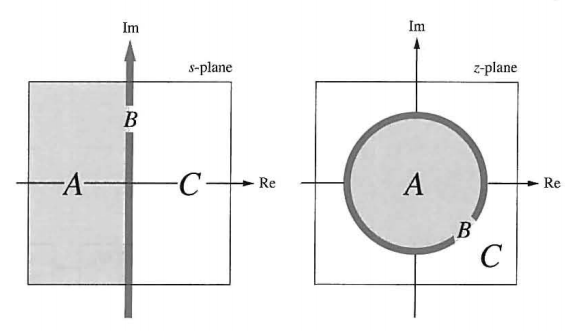
\includegraphics[width=0.7\linewidth]{plano_estabilidade_digital}
	\caption{Regiões do plano s mapeadas no plano z}
	\label{fig:planoestabilidadedigital}
\end{figure}

Desta forma um sistema de controle digital pode ser, estável, se todos os polos do sistema em malha fechada se encontram dentro do círculo unitário do plano z, instável, se existir ao menos um polo fora do círculo unitário ou se houver polos de multiplicidade maior que um em cima do círculo, e marginalmente estável se houver polos de multiplicidade um em cima do círculo unitário e os outros polos se encontrarem dentro do círculo.

% Fim Capítulo















